\documentclass[twocolumn,letterpaper,10pt]{article}
%\usepackage[T1]{fontenc}
\usepackage{amsmath}
\usepackage{listings}
\usepackage{booktabs}
\usepackage{url}
% The following is needed in order to make the code compatible
% with both latex/dvips and pdflatex.
\ifx\pdftexversion\undefined
\usepackage[dvips]{graphicx}
\else
\usepackage{graphicx}
\DeclareGraphicsRule{*}{mps}{*}{}
\fi

\newcommand{\naive}{na\"{\i}ve }


\title{CSEE4824 Course Project}
\author{Danqing Hua $<dh2604@columbia.edu>$\\
  Jiacheng Yang $<jy2522@columbia.edu>$}
\date{December 2012}

\begin{document}

\maketitle

\section{Introduction}
\label{sec:intro}

In this report, we describe our work towards the course project in
CSEE4824 Computer Architecture 2012 Fall. In this project, we are asked to optimize for a specific matrix
operation workload and to design a computer architecture for this
workload.

We focus our optimization on standard matrix multiplication
algorithm. We aim to optimize our code in an architecture-sensitive
way, such that we fully exploit the ILP and TLP in hardware.

We start our architecture configuration from a single-core design. After that, we find
another multi-core design and compare these two options.

Our report is structured as follows. In Section ~\ref{sec:software}, we introduce our software optimization
techniques. Section ~\ref{sec:design} explains how we explore the
design space in a systematic way. We show our experimental results on
both software optimization and architecture tuning in Section
~\ref{sec:exp}. We conclude our report in Section ~\ref{sec:conclude}.

\section{Software Optimization}
\label{sec:software}

Among the four matrix operations, matrix
multiplication dominate the computation cost in this workload.
Thus, we follow the Amdahl's law to optimize this operation first.

Standard matrix multiplication has $O(n^3)$ complexity. Strassen
algorithm~\cite{CLRS} is a well-known algorithm which has a lower
complexity of $O(n^{2.81})$. However, Strassen algorithm is not applicable to our problem. First, the test
case is not big enough to cover the constant factor in Strassen
algorithm. The biggest test case is of size 201, $201^3 = 2.73 *
201^{2.81}$. In order to make Strassen algorithm faster, the
constant cannot be more than 2.73. The additional work
to apply the Strassen algorithm, e.g. padding the matrix with 0, malloc
temporary matrix and recursive function call is overwhelming. Second, Strassen is not
easy to parallelize. Thread spawning are required in a child thread,
which is not supported by $SESC$.

So we focus on optimizing standard matrix
multiplication algorithm, but in an architecture-sensitive way.

\subsection{Loop Ordering}
First of all, for matrix multiplication, there are mutliple ways to order the
loops. We choose the i,j,k ordering, because
we can use a register to store the temporary result
$r(i,j)$. Other ordering may enable us to reference elements in input
matrix A or B by registers. However, in general memory write is more
costly than memory read, so it's better for us to buffer the
write into a register. With this ordering, we also benefit from
spatial locality in both input matrices after we transpose matrix $B$.

\subsection{Transpose Matrix B}
In i,j,k ordering, the data access to matrix $B$
in the inner loop is not sequential. It reads $B$ with a stride length
of $n$. If no optimization is made, it will
introduce more cache misses, even TLB misses. We transpose the matrix $B$ in advance, so that the access to matrix $B$ is sequential.

\subsection{Loop Unrolling and Register Reusing}
Loop unrolling has at least the following
two advantages: (1) reduce branches (2) reuse registers to avoid memory
access. By loading a common value used in an outer-loop in a register,
we avoid fetch the data repeatedly from L1 or L2 caches~\cite{revisited,berkeley}. Combining
loop unrolling and register reusing gives us a speedup of 1.5.

In our implementation, we have two layers of loop unrollings. The first
is to unroll the inner-loop (indexed by $k$). But what is more
important here is that  we also unroll the outer-loop (indexed by $j$). Because
the inner-loop is tight, we still have abundant available
registers. If we use registers as another memory hierarchy~\cite{revisited},
we can further speed up our program. Meanwhile, although the access to
$a(i,k)$ in the inner-loop is not replaced by a register, since we
organized the code in a compact way, the value of $a(i,k)$ is likely
to be kept in a register, so a large number of memory traffic is
saved.

\subsection{Cache Blocking}
Cache blokcing is a technique to improve cache behavior of matrix
multiplication~\cite{block}. Basically, it breaks down the matrix into
cache-size blocks. It uses a block as much as
possible after loading it from memory. The ideal block size is
the maximum block size that can hold the entire blocks in L1/L2 cache. It
is given by~\cite{davis},
\begin{equation}
  2 * BlockSize^2 * wordSize = L1\ Cache\ Size
\end{equation}

If we use a 16K L1 cache, the block size is 32. Additionally, we also
like the block size to be a multiple of the cache-line size.

We implemented the cache blocking algorithm, but the experiment shows
us that the saving effect of cache blocking is not significant. Instead, it performs even worse than non-blocking
algorithm, even if the simulation result shows a lower L1 miss rate.

The reason for this degradation is that the miss penalty of L1 miss
is too small. Even if we use a huge L2 cache with 1M cache size, the
access time to this cache is only 2-3 cycles. Meanwhile, such a small miss
penalty is very likely to be hidden by instruction-level
parallelism. We also tried to optimize cache blocking to alleviate L2
cache miss. However, it seems that L2 miss is also not the bottleneck of
our performance, at least from our experiment (see Section ~\ref{sec:design}).

In fact, cache blocking counteracts with the advantage of
register reusing. We have to write the result matrix multiple times
with cache blocking. Similar conclusion can be found in
~\cite{revisited}, it suggests to trade L1 reuse for register utilization.

We verify our idea by increasing the access time of L2 cache (instead
of using the given formula). With increased miss penalty, cache
blocking version becomes more efficient (see Section ~\ref{sec:exp}).

\subsection{Multi-threading}
We use multi-threading to achieve thread-level parallelism. We evenly partition the rows of
the output matrix. Each thread works to compute the rows
that are assigned to it. There is neither skewness nor race condition in such
partition. Our experiment in Section ~\ref{sec:exp} shows that our multi-threading implementation achieves a linear speed-up.

\subsection{Optimizing other operations}
The techniques used to optimize the other three operations are
basically the same as matrix multiplication, namely loop unrolling,
register reusing and multi-threading.

What's worth mentioning is that the access pattern of these three
operations are simple. For
scaling and addition, data is read only once, so there is no
temporal locality here, but we benefit from spatial locality
especially when the cache-line size is large.

For matrix-vector multiplication, the matrix is read once, while the
vector is read multiple times. But the vector size in the large test
case is only 201. Suppose one cache line is left for the matrix, and one cache line
is left for the output vector. Our L1 cache is big enough to hold the
entire vector. Thus, we do not optimize specifically for the cache
behavior of matrix-vector multiplication.


\section{Exploring the Design Space}
\label{sec:design}

The general principle of our exploration is that we start from simple
parameters. We gradually fix more parameter and tune for an unknown
parameter. Lessons from the architecture course greatly helps us reduce the search space.

\subsection{Single-core}
We start exploring the design space from a single-core design. Let's
first assume that we've figured out the best cache configuration.

\paragraph{Inorder v.s Out-of-order:} Our intuition is that
out-of-order is much better than inoder execution because of ILP. We
verify this by the following micro-benchmark on a large test case.

The result clearly demonstrates the advantage of out-of-order
execution over in-order execution, even if the issue width of the
out-of-order execution is only 1.

\begin{table}[ht!]
\begin{center}
\begin{tabular}{ccccc}
\toprule
Execution   &  Freq  & Issue width  &  time  & power \\
\midrule
In-order   &  1G  &  1  &  2527  &  4.6 \\
Out-order     &  1G &  1  &    594 & 14.3 \\
\bottomrule
\end{tabular}
\end{center}
\caption{Comparing in-order and out-of-order}
\end{table}

The power of out-of-order execution is much higher than in-order execution. In-order execution
consumes less power because most of its time is spent on stall. From
the detailed power consumption, we can tell that a
large part of its power is spent on clock instead of on execution. So
power utilization of in-order exeuction is actually lower. Thus, we adhere our following exploration to out-of-order execution.

\paragraph{Issue width:} Issue width influences the instruction-level
parallelism we can achieve. We speculates that a larger issue width
will give us better performance.

On a moderate size test case, we fix all other parameters and vary the issue
width. The result in Figure ~\ref{fig:issue} shows that as the issue width
becomes larger, the execution is faster. But after issue width
is larger than 4, the performance stops improving on all types of cores. We conclude that the
instruction-level parallelism is fully exploited in such cases. Continuing
increasing issue width will only increase the cost of maintenance, such as the access time to the re-order buffers.

\begin{figure}[ht!]
\begin{center}
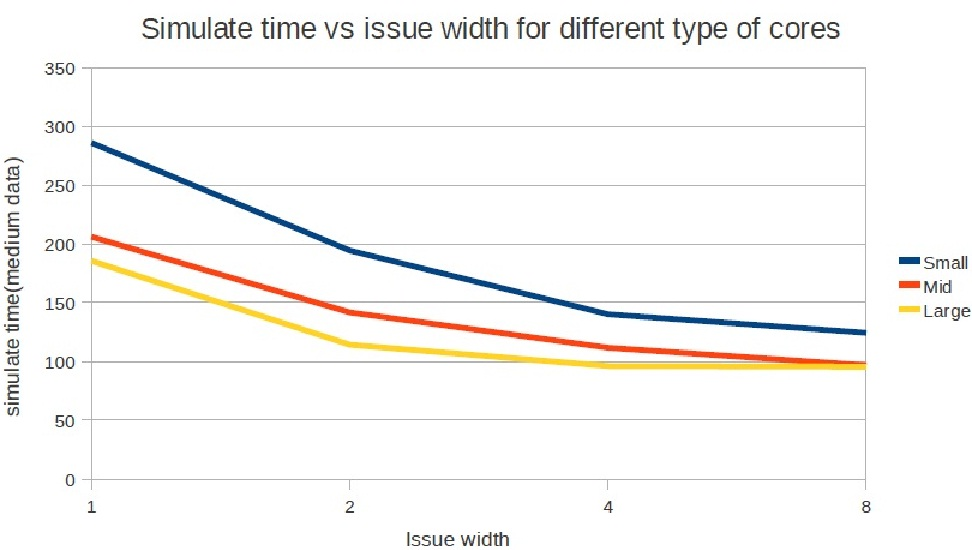
\includegraphics[width=0.4\textwidth]{figures/issue.jpg}
\end{center}
\label{fig:issue}
\caption{Simulation time V.S issue width}
\end{figure}

\paragraph{Type of cores:} At a first glance, large core may be the
first choice, as it carries more powerful functional units. However,
we have to lower the frequency to meet the power
constraint. There is no clear good or bad in choosing the type of
cores. Each type of core can achieve a good performance with
appropriate parameters. Some
preliminary experiments let us prefer SmallCore and MidCore because
of their relative high performance/power efficiency.

We dismiss the idea for a heterogeneous multi-core architecture,
because this workload can be partitioned into equal size. It
doesn't make sense to bias one thread or another by giving it a more
powerful core.

\paragraph{Frequency} The guideline for tuning frequency is: as
high as possible within the power constraint. So we usually tune the
frequency after all other parameters are fixed.

\subsection{Multi-core}
Our experiment shows
that our program has a linear speed-up. So having more
cores presumably is better. Considering the power constraint, we
focus on a dual-core architecture to illustrate what is new in
a multi-core architecture.

An interesting observation is about the power
efficiency of multi-core architecture. We measure the power efficiency of an architecture as Performance per
Watt. Performance is measured by KIPS (kilo-instructions-per-second)
from $SESC$'s result. We plot the power efficiency of architectures
with different number of cores. We can see in Figure ~\ref{fig:power} that as the number of cores
increases, the power efficiency also increases.

\begin{figure}[ht!]
\begin{center}
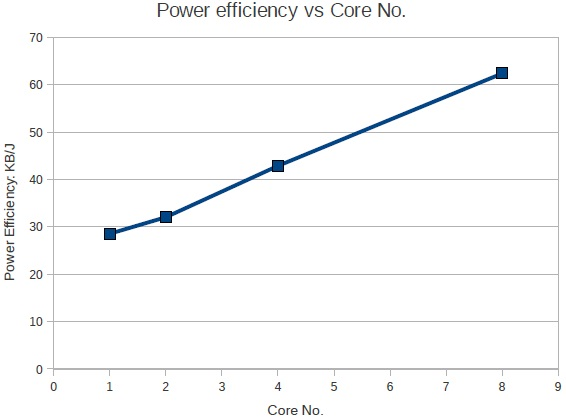
\includegraphics[width=0.4\textwidth]{figures/efficiency.jpg}
\end{center}
\caption{Power efficiency V.S number of cores}
\label{fig:power}
\end{figure}

\subsection{Configuring Cache}

\subsubsection{Cache Hierarchy}
For single core architecture, a two-level cache hierarchy is a better
choice. L1 cache guarantees fast access, while the larger L2 cache stores
more data to avoid the penalty of memory access.

For multi-core architecture, we choose a shared-L2 hierarchy. 
In our workload, matrix $B$ is shared by all
threads. Using a private L2 cache will only lead to unnecessary cold
start.  

\subsubsection{L1 Cache}
Our code is very small, so we don't need a large L1 instruction
cache. We fix L1 instruction cache to its minimum size 16K. L1 data
cache is chosen to 16K as well, mainly because it saves power and L2
cache access is cheap.

\subsubsection{L2 Cache}
Unlike L1 cache, whose size has a significant influence on
power. Enlarging L2 cache seems to come for free. We vary the size of
L2 cache from 16K to 1M, the power remains stable, and the access
time is within 3 cycles. The total size of three matrices is $201 *
201 * 3 * 8 = 946K$, so a 1M L2 cache can hold almost every
data. Misses in L2 cache in this case are due to compulsory misses
during matrix generation or conflict misses.

Furthermore, we notice that the size of L2 actually doesn't have much
impact on our performance. Having a 16K L2 cache only leads to a
6\% performance drop versus 256K L2 in our final configuration (from
100 msec to 106 msec). We assume it is because the
access time to memory in the simulator is small, and the DRAM access
is low with our optimization.

\subsubsection{Cache block size}
Because almost all reads are sequential in this workload, we prefer a larger cache-line size. We set the block size to 64
bytes, because it guarantees a low access time for L1 cache and it won't
bring in too much unnecessary data at the boundary of a row or a partition.

\section{Experiment}
\label{sec:exp}
In this section, we illustrate some experimental results to support
our claims in Section ~\ref{sec:software} and Section ~\ref{sec:design}.
 
\subsection{Cache Blocking}
We mentioned in Section ~\ref{sec:software} that cache blocking does not give us
too much performance gain. Instead, it hurts our performance.

First, we show the result by varying block size in a
single-core configuration: 1.8 GHz MidCore, issue width = 2. The L1
cache is 16KB, and the L2 cache is 1M, block size is 64 bytes. The
workload is medium. The start-up time in main the function(e.g. matrix
generation) is roughly 1.9 msec.

Here, we find the following observations (1) the best block size is
smaller the ideal block size we calculated before (2) in our workload,
the performance downgrades with blocking. The block size should be
smaller because of conflict in L1 cache.

\begin{table}[ht!]
\begin{center}
\begin{tabular}{ccccc}
\toprule
blocksize & time & L1 miss & L2 miss & \%Dram \\
\midrule
16 & 6.944 & 0.67	 & 12.21	& 0.53 \\
24 & 6.682 &  1.01 &	8.54	& 0.80 \\ 
32 & 6.711 & 1.66	 & 5.19	& 1.31 \\ 
40 & 6.585 &  1.89 & 4.70	& 1.48 \\ 
None	& 6.514	& 1.78 & 5.08	& 1.40 \\
\bottomrule
\end{tabular}
\end{center}
\label{fig:blocking}
\caption{Cache blocking: Effect of block size}
\end{table}

To see when the cache blocking algorithm works, we increase the
access time of L2 cache. When the gap between L1 cache and L2 cache increases, 
cache blocking becomes more important. Blocking will have more effect
in reducing L2 cache miss, supposing the gap between L2 and memory is
large, say hundreds of cycles. However, it seems in this simulator the
gap between L2 and memory is not large enough either (see above Section).

\begin{table}[ht!]
\begin{center}
\begin{tabular}{cccc}
\toprule
L2 access time & Ideal	& Nonblocking & Speedup\\
\midrule
3 &	6.682 & 6.514 & 0.97 \\ 
30 & 6.899  & 7.168 & 1.04 \\ 
50	& 7.082	& 8.036 & 1.13  \\ 
100	& 7.589	& 10.647 & 1.40 \\ 
200	& 8.624	& 15.888 & 1.84\\
\bottomrule
\end{tabular}
\end{center}
\caption{Cache blocking: Effect of L2 access time}
\end{table}


\subsection{Loop Unrolling}

Not let's look at the effect of loop unrolling and how we choose the
best number of unrollings we made based on our experiment. It is clear
from the result that unrolling the $j$ loop 2 times is the best
choice. As the unrolling times reaches 3, the performance drops,
because we have used up all the registers, and we will have a register
thrashing here. The inner-most loop can be unrolled 4 times or 2 by
changing a switch in the code.

\begin{table}[ht!]
\begin{center}
\begin{tabular}{ccccc}
\toprule
Unrolling & time & L1 miss  & L2 miss & Speedup \\
\midrule
None & 10.211 & 1.93 & 5.04	& 1.3 \\
1 & 6.821 & 1.81 & 5.08 & 1.38 \\
2 & \textbf{6.515} & 1.78 & 5.08 & \textbf{1.4} \\
3 &	6.59 & 1.64	& 5.08 & 1.42 \\
\bottomrule
\end{tabular}
\end{center}
\caption{Speedup of loop-unrolling}
\label{fig:unrolling}
\end{table}


\subsection{Multi-threading}

We test the scalability of our multi-threading program. Our configuration is $n$ MidCore with issue width 2, we vary $n$. Each core
has 16K L1 Instruction cache and 32K L1 Data cache. The L2 shared
cache is 256K. We use out-of-order execution and set the frequency to
1.8GHz. We run this test on medium (we substract the start-up time in
the main function).

When we scale the number of cores from 1 to 4, it has a linear
scale-up. When the number of threads reaches 8, the speedup a
sub-linear. Adding more threads increases coordination cost and will
saturate common memory bus if the program is bound by memory bandwidth. And we will suffer from skewness, i.e. the
execution is limited by the slowest thread. So we cannot scale up linearly with too many threads.

\begin{figure}[ht!]
\centering
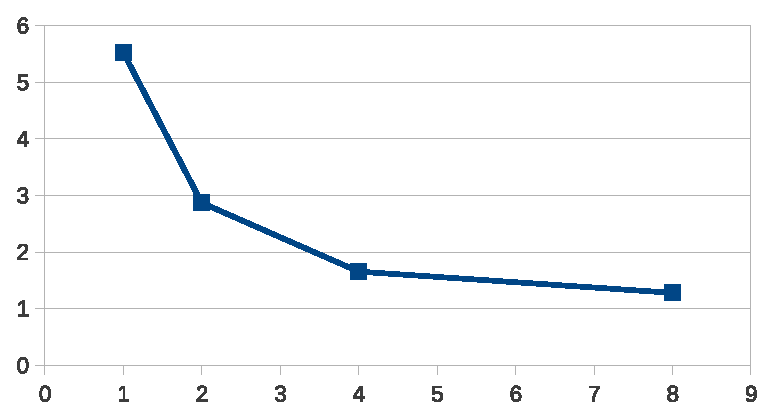
\includegraphics[width=0.4\textwidth]{figures/scale2.eps}
\caption{Scaling with more threads}
\end{figure}

\subsection{Final Performance}
We report the final performance of our architecture and program. We
present two configurations here, one for single-core architecture and the
other for multi-core architecture. The configurations for both architectures
are shown in Table ~\ref{table:config}. The results are reported in Table ~\ref{table:single} and Table ~\ref{table:multi}.

\begin{table}[ht!]
\begin{center}
\begin{tabular}{ccccc}
\toprule
& Single & Multi \\
\midrule
Core type & Mid & Small \\
Inorder & false & false \\
Issue width & 2 & 2 \\
Frequency & 2.1G & 1.6G \\
Cache Org & L2Single & L2Share \\
L1 Cache & 16K & 16K \\
L2 Cache & 512K & 256K \\
Block size & 64 & 64 \\
\bottomrule
\end{tabular}
\end{center}
\caption{Final configurations}
\label{table:config}
\end{table}

\begin{table}[ht!]
\begin{center}
\begin{tabular}{ccccc}
\toprule
Test  & time & L1 miss & L2 miss & Power \\
\midrule
Small & 0.606 & 0.29 & 56.76& 25.131 \\
Medium  & 5.585 & 1.78 & 5.08 & 27.907 \\
Large & 100.055 & 1.89 & 5.97 & 29.493 \\
\bottomrule
\end{tabular}
\end{center}
\caption{Single-core final result}
\label{table:single}
\end{table}


\begin{table}[ht!]
\begin{center}
\begin{tabular}{ccccc}
\toprule
Test  & time & L1 miss  & L2 miss & Power \\
\midrule
Small &  0.725 & 0.28 & 65.21 & 22.447 \\
Medium  & 5.9 & 1.6 & 9.77 & 27.505 \\
Large  & 103.247 & 1.64 & 95.82  & 29.848 \\
\bottomrule
\end{tabular}
\end{center}
\caption{Multi-core final result}
\label{table:multi}
\end{table}

There is no clear winner between a single-core and multi-core design. In this application, there is
abundant instruction-level parallelism: instructions and data are
mostly independent, data dependency is less. With software
optimization,  we can exploit ILP to the
extreme. Single-core architecture is also more simple and
efficient. We tried to use `L2Shared' model with one thread, and it performs
much worse than the `SingleL2' model. Although our multi-core architecture does not win over the single-core
design within this power constraint, by our experiment, we show that
our algorithm design is scalable with the number of cores.

\section{Conclusion}
\label{sec:conclude}

In this report, we summarize our techniques to optimize matrix
operations. We use pre-processing, software loop-unrolling,
register reusing to enhance the execution of single thread
execution. We apply multi-threading to
parallelize all four operations and achieve a linear scale-up.

We systematically explore the design space, finding out the best
architecture for both uni-core and dual-core
architecture. Instead of enumerating all possibilities in the design
space, our search is guided by our understanding in architecture
concept.

Finally, we experimentally verify our design and quantify the speedup
in our software optimization.

\bibliographystyle{abbrv}
\bibliography{refs}

\end{document}
